\documentclass{article}
\usepackage{setspace}
\usepackage{listings}
\usepackage{color}
\usepackage{xcolor}
\usepackage{geometry}
\usepackage{graphicx}
\usepackage{booktabs}
\usepackage[normalem]{ulem}
\usepackage{tabularx}
\usepackage{hyperref}
\usepackage{enumitem}
\geometry{a4paper,bindingoffset=0.2in,%
	left=1in,right=1in,top=1in,bottom=1in,%
	footskip=.25in}

\onehalfspacing

%opening
\title{MECHTRON 4TB6: Requirements Specification \\ LifeLine}
\author{Group 30 \\ Emily Crowe, crowee \\ Arthur Faron, farona \\ Danushka Fernando, fernad12 \\Yerin Thevarajah, thevaryn \\ Phillip Truong, truonp1}

\usepackage{enumitem}
\usepackage{natbib}
\begin{document}

    \date{October 24, 2021}
	\maketitle
	\newpage
    
	\tableofcontents
	\listoffigures
	\listoftables
	\newpage

	\section{Scope}
	\subsection{The Purpose of the Project}
	\paragraph{}
	When first responders or first-aiders respond to emergencies and encounter at-risk casualties out in the field, they are put into stressful situations with unknown first aid resources. With only limited knowledge and means of qualitative measurements, vital signs can only be recorded mentally and communicated verbally to either emergency medical technicians (EMTs) or hospitals. Due to this, there can be inaccurate transfer of information. 
	\paragraph{}
	There are two components of responding to a first-aid situation: The Primary Survey which includes checking airway, breathing, circulation, and any treatment for immediate life-threatening situations that can be done before the ambulance arrives. However, if the ambulance arrival is delayed due to external circumstances, there needs to be a secondary survey to assess the casualty in more depth and treat them accordingly. This includes taking vital signs, such as body temperature, blood pressure, and heart rate, which would help the first-aiders assess the situation and decide on the best course of action to take with regards to treatment based on the observed results. 
	\paragraph{}
	The project, named LifeLine, intends to help a first-aider monitor a casualty's vital signs to keep them stable until emergency medical services (EMS) arrives. This project also intends to assist a first-aider by retrieving vital signs quantitatively. These results can then guide the first-aider to adapt and improve their treatment plan. The device is able to record and save the vital sign data which can later be exported for more advanced analysis by medical professionals.
	
	\subsection{The Scope of the Project}
	\paragraph{}
	LifeLine is a product that carries out four (4) primary functions: quantitative measurement of primary vital signs through sensor readings, logging the primary vitals data, displaying the primary vitals data, and exporting the primary vitals data. The primary vital signs this project will be measuring are body temperature, blood pressure and heart rate. 
	\paragraph{}
	The device will instruct the user where to place the different sensors for each vital sign in order to measure them safely and efficiently. While these procedures are taking place, the device will present the results on a display. The first-aider can use this to further their treatment and continue monitoring the vital signs until medical assistance arrives. The product will then log the measurements and export this data into an accessible file to be used for medical records and for further examination by medical professionals. 
	
	\subsection{Out of Scope: Future Development}
    \paragraph{}
    A smartphone application to record the results of the vital signs and analyze them through the application is a possible extension of this project. This application would be able to give the first-aider suggestions for possible diagnoses and immediate treatments using the data collected by the device.
    \paragraph{}
    The scope of this project can be expanded further in the future by improving the data transfer between first-aiders and emergency medical technicians. By integrating the smartphone application with the data collection system used by EMS and hospitals, the casualty's data can be passed on quickly and accurately.
    \paragraph{}
	Due to time limitations, it was decided to reduce the scope of the project to focus on creating a device with sensors to take vital signs, display them, and transfer the data for future use as a proof-of-concept.
	
	\newpage
	\subsection{Naming Conventions and Terminology}
    \paragraph{General Terminology}
	\begin{itemize}
	    \item User : Person using the LifeLine device. 
	    \item First aid qualifications: Emergency and Standard CPR, Medical First Responders \citep{sja}.
	    \item Sensor: A device that measures physical input from its environment and converts it into data that can be interpreted by either a human or a machine. Most sensors are electronic but some can be analog such as a glass thermometer \citep{sensor}. 
    \end{itemize}
    
	\paragraph{First Aid Terminology}
	\begin{itemize}
	    \item First responders: EMS, firefighters, paramedics, or police officers.
	    \item First aid:  Emergency care given to an individual in the case of serious injury with the aim to keep the individual alive and prevent further injury.
	    \item First-aider: Individual performing first aid.  For instance, a person trained in first aid arriving on a scene to treat an injured person.
	     \item Casualty: Individual receiving first aid treatment.
	    \item EMS: Emergency Medical Services.  Paramedic or ambulatory services that have been called to respond to a situation. 
	    \item EMT:  Emergency Medical Technician.
	    \item 911:  Emergency telephone number in Canada.
	    \item CPR:  Cardio Pulmonary Resuscitation.  A method delivering mouth-to-mouth resuscitation and artificially pumping blood during cardiac arrest.
	    \item ABC:  Airway, Breathing, Circulation.  Acronym used by first-aider to remember the sequence of performing CPR.
	    \item Primary Survey:  Initial assessment of casualty.  The Primary Survey is used to identify and treat life-threatening injuries as well as prevent any further complications. Also known as ABC's.
    \end{itemize}
    
	\paragraph{Medical Terminology}
	\begin{itemize}
	    \item Heart rate:  Number of heart beats per minute.  Measured in BPM.
	    \item Pulse:  Same as the heart rate, number of heart beats per minute.  Also measured in BPM.
	    \item BPM:  Beats per minute.  Unit used to measure heart rate in a clinical setting.
	    \item Blood pressure:  The pressure on arteries both when the heart beats and between heart beats.  Comprised of systolic and diastolic blood pressure respectively.  Measured in mmHg.
	    \item mmHg: A unit of pressure equal to the pressure exerted by a column of mercury 1 millimeter high at 0°C.  Unit used to measure blood pressure in a clinical setting. 
	    \item Systolic blood pressure:  The pressure on arteries when the heart beats and pumps blood out to the arteries.
	    \item Diastolic blood pressure:  The pressure on arteries between heart beats when the heart is at rest.
	    \item Vitals: The four vitals are body temperature, blood pressure, heart rate, and respiration rate. Vital signs are used to detect and monitor medical issues. 
	    \item Carotid artery: Major artery that supplies blood to the brain. Typically it is used in first aid since it is a large artery and located near the surface of the skin.
	    \item Cardiac arrest: Occurs when the heart stops beating.  Without a beating heart, blood cannot be pumped to the rest of the body.  Since oxygen is delivered to organs through the blood, the lack of oxygen can be fatal. 
	    \item Shock: Sudden drop in blood flow to organs that can be life-threatening. Because shock can accompany many serious illnesses or injuries, it is important to treat shock while performing first aid.


	\end{itemize}
	\newpage
	\subsection{Relevant Facts and Assumptions}
	
	\subsubsection{Current Methods of Performing First Aid}
	
	Common situations requiring first aid treatment:
	\begin{itemize}[noitemsep]
	    \item Allergic reactions
	    \item Burns
	    \item Bleeding
	    \item Cardiac arrest
	    \item Head injury
	    \item Poisoning
	    \item Shock 
	    \item Seizures
	    \item Stroke
	\end{itemize}
	
	When a first-aider arrives on the scene and conducts the Primary Survey, the acronym ABC is used to evaluate a casualty's situation. This refers to checking a casualty's airway, breathing, and circulation. To check a casualty's airway and breathing, the current method is to tilt the head to clear the airway and look at the casualty's chest while listening and feeling for breaths.  This method is quick and effective for determining whether a casualty is breathing or not breathing.    
	\paragraph{}
	To check a casualty's circulation, a first-aider places two fingers on the carotid artery to feel for a pulse.  The first-aider is required to check pulse every minute until EMS arrives at the scene.  
	\paragraph{}
	Although situations such as head injury, burns, or bleeding, may not directly impact a casualty's airway, breathing, or circulation, shock often accompanies serious injury. Shock causes the blood flow to organs to slow down which can result in loss of consciousness and can be life-threatening in severe cases.  For this reason, it is important for the first-aider to continually monitor a casualty's vital signs.  
	\paragraph{}
	Both hypothermia and heat stroke are associated with extreme changes in body temperature.  Signs of hypothermia typically include shivering and skin that is very cold to the touch \citep{hypothermia}.  Signs of heat stroke include a high body temperature, flushed skin, and a rapid heart rate \citep{heartrate}.  However, these two conditions may be difficult to identify if the casualty has other injuries as well.  For both hypothermia and heat stroke, the longer the treatment of warming or cooling the body is delayed, the likelihood of serious complications increases.
	\paragraph{}
	A significant drop in blood pressure can cause fainting and loss of consciousness. Therefore it is an important sign to monitor and could be indicative of underlying problems such as significant bleeding, severe infection, or allergic reaction.
	\paragraph{}
	In Canada, a first-aider can only stop administering first aid when another person takes over performing cardiopulmonary resuscitation (CPR), when emergency medical services (EMS) arrives, or when it is unsafe to continue. 
	\paragraph{}
	Primarily, first-aiders are focused on life threatening injuries and are looking to assess whether a casualty is breathing or not breathing. Since the current methods are effective, the LifeLine device will not measure respiration rate. 
	\paragraph{}
    Volunteers of St. John Ambulance \citep{sja} record any information gathered on an Incident Report. However, due to time constraints, information is collected through notes and sometimes memory. This is usually given to the EMT's when they arrive.
    \paragraph{}
    For the operation of this device, casualty is assumed to be an adult. In first aid, this is considered anyone above the age of 12 \citep{redcross}.

	\newpage

	\subsection{Behaviour Overview}
    The three vitals: body temperature, blood pressure, and heart rate, will be measured and passed to the microcontroller as shown in Figure \ref{module}.  During the design process, the appropriate sensor for each vital will be selected.  A microcontroller will be used to process the data received from the three sensors.  Additionally, the requirements for the memory of the device are specified in \ref{mem}  Power Supply requirements are further outlined in \ref{power_1} and \ref{power_2}.  The microcontroller will export all processed data to the display.  The display will allow the user to monitor the vitals of the casualty.
    
    \begin{figure}[!htb]
    	\centering
    	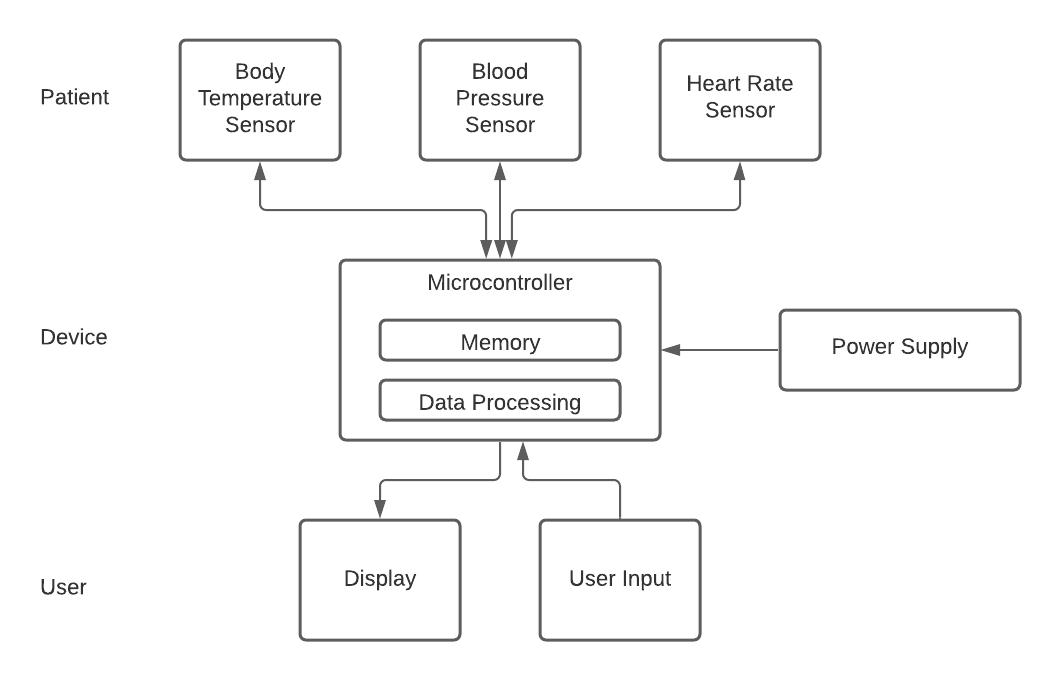
\includegraphics[width=0.75\linewidth]{LifeLine block diagrams - Page 1.png}
    	\caption{High level module diagram outlining the main components used in the LifeLine device and how they interact with the casualty and user. }
    	\label{module}
    \end{figure}
    
    The data flow from casualty to user is outlined in Figure \ref{dataflow}.  Out of range detection is used to identify whether the readings are physically possible.  The display alerts the user if one or more of the vitals (body temperature, blood pressure, heart rate) are outside of the acceptable range.  Vital status tells the user whether the vital is within range.
    
    %add paragraph with ref
    \begin{figure}[!htb]
    	\centering
    	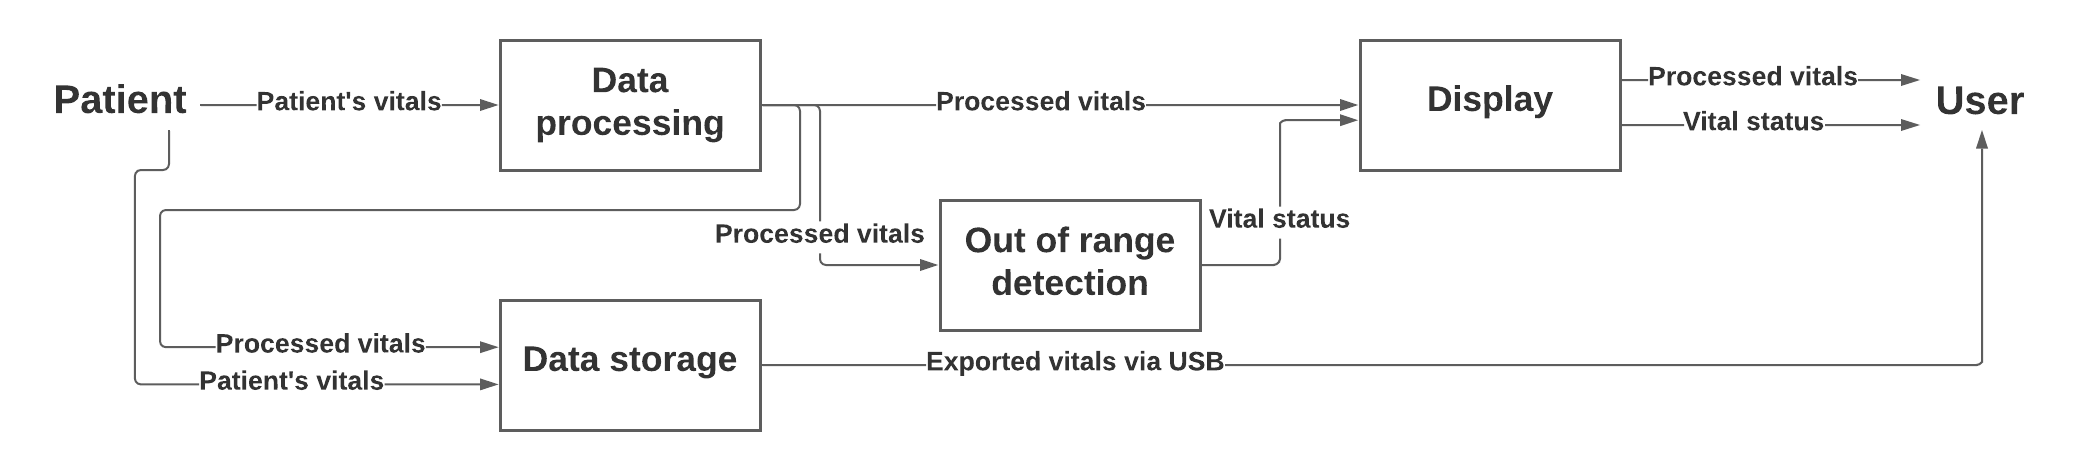
\includegraphics[width=1\linewidth]{Data flow final.png}
    	\caption{Data flow diagram outlining how the casualty's vitals (body temperature, blood pressure, heart rate) are processed, stored, and displayed.}
    	\label{dataflow}
    \end{figure}
    
 
    \newpage
    
    \section{Variables}
    \subsection{Monitored Variables}
    
        \begin{table}[hbt!]
        \caption{Monitored Variables} 
        \begin{tabular}{|l|l|l|l|}
        \hline
        Variable name  & Description                                                                                   & Type of Variable & Units          \\ \hline
        m\_BT\_casualty & \begin{tabular}[c]{@{}l@{}}Body Temperature recorded by \\ sensor pre-processing\end{tabular} & Monitored        & Degree Celsius \\ \hline
        m\_BP\_casualty & \begin{tabular}[c]{@{}l@{}}Blood Pressure recorded by \\ sensor pre-processing\end{tabular}   & Monitored        & mmHg           \\ \hline
        m\_HR\_casualty & \begin{tabular}[c]{@{}l@{}}Heart Rate recorded by \\ sensor pre-processing\end{tabular}       & Monitored        & BPM            \\ \hline
        \end{tabular}
        \end{table}
    
    \subsection{Controlled Variables}
    \begin{table}[hbt!]
    \caption {Controlled Variables}
    \begin{tabular}{|l|l|l|l|}
    \hline
    Variable name   & Description                                                                                                                                 & Type of Variable & Units          \\ \hline
    c\_BT\_disp     & \begin{tabular}[c]{@{}l@{}}Body Temperature after data\\ processing displayed on device\end{tabular}                                        & Controlled       & Degree Celsius \\ \hline
    c\_BP\_disp     & \begin{tabular}[c]{@{}l@{}}Blood Pressure after data\\ processing displayed on device\end{tabular}                                          & Controlled       & mmHg           \\ \hline
    c\_HR\_disp     & \begin{tabular}[c]{@{}l@{}}Heart Rate after data processing \\ displayed on device\end{tabular}                                             & Controlled       & BPM            \\ \hline
    c\_BT\_sensorOK & \begin{tabular}[c]{@{}l@{}}Indicates whether the readings from \\ the body temperature sensor are within\\ an acceptable range\end{tabular} & Controlled       & Boolean        \\ \hline
    c\_BT\_sensorOK & \begin{tabular}[c]{@{}l@{}}Indicates whether the readings from\\ the blood pressure sensor are within an\\ acceptable range\end{tabular}    & Controlled       & Boolean        \\ \hline
    c\_BT\_sensorOK & \begin{tabular}[c]{@{}l@{}}Indicates whether the readings from \\ the heart rate sensor are within an \\ acceptable range\end{tabular}      & Controlled       & Boolean        \\ \hline
    \end{tabular}
    \end{table}
    
    \newpage 
    
    \subsection{Constants}
    \begin{table}[hbt!]
    \caption {Constant Variables}
    \begin{tabular}{|l|l|l|l|}
    \hline
    Variable name  & Description                                                                                                                                 & Type of Variable & Units          \\ \hline
    k\_BT\_range   & Acceptable body temperature range                                                                                                           & Constant         & Degree Celsius \\ \hline
    k\_BT\_range   & Acceptable blood pressure range                                                                                                             & Constant         & mmHg           \\ \hline
    k\_HR\_range   & Acceptable heart rate range                                                                                                                 & Constant         & BPM            \\ \hline
    k\_SetupTime   & \begin{tabular}[c]{@{}l@{}}Amount of time to set up the device \\ and place sensors on the casualty\end{tabular}                             & Constant         & Seconds        \\ \hline
    k\_StartTime   & \begin{tabular}[c]{@{}l@{}}Amount of time from when the device\\ is powered on to when the device starts \\ monitoring vitals.\end{tabular} & Constant         & Seconds        \\ \hline
    k\_RefreshRate & \begin{tabular}[c]{@{}l@{}}The rate at which the display will be updated\\ with a new reading\end{tabular}                                  & Constant         & Hz             \\ \hline
    \end{tabular}
    \end{table}

    \newpage
    \section{Requirements}
    \subsection{Functional Requirements}

     \begin{enumerate}[label = \textbf{{FR}\arabic*}  ]
     
         \item The device shall have an "ON" and "OFF" button to power up and power down the device.
    	  	    \begin{itemize}
    	  	        \item Rationale:  When the device isn't used, it should be powered off to conserve the power supply.  
    	  	        \item Criterion: There is a button on the device that powers it up and down.
    	  	    \end{itemize}
    	  	    
    	 \item The device shall have the option for the user to record vitals of multiple casualties one at a time and differentiate them accordingly.
	  	    \begin{itemize}
	  	        \item Rationale:  If a first-aider were to use the LifeLine device in a situation with multiple casualties, each casualty's vitals should be kept separate.   
	  	        \item Criterion: The device shall have the option for the user to record vitals of multiple casualties one at a time and differentiate them accordingly.
	  	    \end{itemize}
	  	
	  	\item \label{power_1} The device must be capable of operating uninterrupted for at least one hour.
	        \begin{itemize}
	            \item Rationale: Provincially legislated response time from the time a call is placed to EMS to when an ambulance arrives is eight minutes \citep{responsetime1}.  However, many municipalities do not meet this criteria up to 25\% of the time \citep{responsetime3} \citep{responsetime2}.  For non-life threatening injuries, response times can be up to one hour \citep{responsetime3}.   
	            \item Criterion: Power supply must be large enough to allow the device to operate for at least one hour. 
	        \end{itemize}     
	   
	   \item \label{power_2} While the device is unused, the power supply shall not decrease below 80\% of the maximum capacity.
	        \begin{itemize}
	            \item Rationale: It is unlikely that a first-aider will need to perform first aid frequently.  The LifeLine device should be functional even after long periods without use.   
	            \item Criterion: Power supply shall not decrease to below 80\% of maximum capacity over the course of one month unused. 
	        \end{itemize}
	        
        \end{enumerate}

        \paragraph{Body Temperature}
        \begin{enumerate}[label = \textbf{{FR5.}\arabic*} ]
        %Body temperature
        \item The device shall have a sensor that measures body temperature.
            \begin{itemize}
                \item Rationale: Body temperature is a vital sign.  Extremely high or low body temperature is a cause for concern and can be life-threatening. 
                \item Criterion: The device shall have a sensor that measures body temperature.
            \end{itemize}
            
        \item The device shall notify the user if the body temperature readings are out of range.
            \begin{itemize}
                \item Rationale: The user should be aware if the body temperature readings are higher or lower than physically possible. 
                \item Criterion: The device shall notify the user if the body temperature readings are out of range.
            \end{itemize}    
            
        \item The device shall clearly communicate the proper placement of the body temperature sensor.
            \begin{itemize}
                \item Rationale: The user should be able to measure the casualty's body temperature without any previous knowledge about how the body temperature sensor works. 
                \item Criterion: The device shall clearly indicate where the body temperature sensor needs to be placed on the casualty.
            \end{itemize}  
        
        \item The device shall process incoming data from the sensor recording temperature to reduce sensor noise.
            \begin{itemize}
                \item Rationale:  Body temperature is unlikely to fluctuate rapidly.  However, noise will be present in the body temperature's signal.  The device will incorporate data processing to ensure the user has an accurate understanding of the casualty's body temperature.
                \item Criterion: The body temperature reading after processing must have less noise than the body temperature reading before processing.
            \end{itemize}
            
        \item The device shall display a casualty's body temperature to the nearest 0.1°C. %CHANGE TO 0.5DEG C FOR THE TEMP SENSOR
            \begin{itemize}
                \item Rationale: A majority of thermometers display temperature to the nearest 0.1°C. 
                \item Criterion: The device shall display the casualty's body temperature to the nearest 0.1°C. 
            \end{itemize}
            
        \item The device shall measure a casualty's body temperature to be accurate within ± 0.5°C.
            \begin{itemize}
                \item Rationale: The difference between the maximum and minimum body temperature in a healthy casualty can be up to 1°C throughout the course of a day \citep{bt1}. 
                \item Criterion: The body temperature reading must be accurate within ± 0.5°C as compared to body temperature measured by oral thermometer. 
            \end{itemize}
        \end{enumerate}
        
        \paragraph{Blood Pressure}
    \begin{enumerate}[label = \textbf{{FR6.}\arabic*} ]
        %Blood Pressure
	    \item The device shall have a sensor that measures blood pressure.
            \begin{itemize}
                \item Rationale:  Blood pressure is a vital sign.  A sudden drop in blood pressure can cause loss of consciousness as well as an increase in blood pressure can indicate extreme stress on the heart \citep{shock}.  Therefore, it is an important sign to monitor when conducting first aid.  
                \item Criterion:  The device shall have a sensor that measures blood pressure.  
            \end{itemize}
	    
	    \item The device shall notify the user if the blood pressure readings are out of range.
            \begin{itemize}
                \item Rationale: The user should be aware if the blood pressure readings are higher or lower than physically possible.   
                \item Criterion: The device shall notify the user if the blood pressure readings are out of range.
            \end{itemize}  
            
        \item The device shall clearly communicate the proper placement of the blood pressure sensor.
            \begin{itemize}
                \item Rationale: The user should be able to measure the casualty's blood pressure without any previous knowledge about how the blood pressure sensor works. 
                \item Criterion: The device shall clearly indicate where the blood pressure sensor needs to be placed on the casualty.
            \end{itemize}  
	    
	   \item The device shall process incoming data from the sensor recording blood pressure to reduce sensor noise.
            \begin{itemize}
                \item Rationale:  Since noise will be present in the blood pressure sensor's signal, the device will incorporate data processing to ensure the user has an accurate reading.
                \item Criterion: The blood pressure reading after processing must have less noise than the blood pressure reading before processing.
            \end{itemize}
	    
	    \item The device shall display the casualty's blood pressure to the nearest 1 mmHg.
	         \begin{itemize}
	            \item Rationale:  Blood pressure is measured to the nearest 1 mmHg. 
	            \item Criterion: The blood pressure reading must be displayed to the nearest 1 mmHg.
	        \end{itemize}
	        
	   \item The device shall measure the casualty's blood pressure to be accurate within ± 10 mmHg.
	        \begin{itemize}
	            \item Rationale: At-home digital blood pressure monitors have a tolerance of 20 mmHg.
	            \item Criterion: The blood pressure reading must be accurate within ± 10 mmHg.
	        \end{itemize}
        \end{enumerate}
        \paragraph{Heart Rate}
    \begin{enumerate}[label = \textbf{{FR7.}\arabic*} ]
	    %Heart Rate 
	   \item The device shall have a sensor that measures heart rate.
            \begin{itemize}
                \item Rationale:  Heart rate is vital sign.  When conducting first aid, first-aiders are required to check the casualty's pulse every minute if they are unconscious. 
                \item Criterion: The device shall have a sensor that measures heart rate.
            \end{itemize}

        \item The device shall notify the user if the heart rate readings are out of range.
            \begin{itemize}
                \item Rationale: The user should be aware if the heart rate readings are higher or lower than physically possible.   
                \item Criterion: The device shall notify the user if the heart rate readings are out of range.
            \end{itemize}  

        \item The device shall clearly communicate the proper placement of the heart rate sensor.
            \begin{itemize}
                \item Rationale: The user should be able to measure the casualty's heart rate without any previous knowledge about how the heart rate sensor works. 
                \item Criterion: The device shall clearly indicate where the heart rate sensor needs to be placed on the casualty.
            \end{itemize}  

        \item The device shall process incoming data from the sensor recording heart rate to reduce sensor noise.
            \begin{itemize}
                \item Rationale:  Since noise will be present in the heart rate sensor's signal, the device will incorporate data processing to ensure the user has an accurate reading.
                \item Criterion: The heart rate reading after processing must have less noise than the heart rate reading before processing.
            \end{itemize}            
	        
	    \item The device shall display the casualty's heart rate to the nearest 1 BPM.
	        \begin{itemize}
	            \item Rationale: Heart rate is measured in BPM.
	            \item Criterion: The heart rate reading must be displayed in BPM to the nearest 1 BPM.
	        \end{itemize}
	        
	   \item The device shall measure the casualty's heart rate with an accuracy of $<$± 10\%.
	        \begin{itemize}
	            \item Rationale:  The acceptable tolerance of heart rate monitors currently on the market such as Apple Watch 3 and Fitbit Charge 2 is ± 10\% \citep{heartrate}. 
	            \item Criterion: The heart rate reading must be displayed within an accuracy of  $<$± 10\%.
	        \end{itemize}
	        
        \end{enumerate}
        \paragraph{Data Transfer and Processing}
        
    \begin{enumerate}[label = \textbf{{FR8.}\arabic*}]
	    \item The device shall have enough hard drive storage to store the vitals (body temperature, blood pressure, and heart rate) for at least two different casualties.
	        \begin{itemize}
	            \item Rationale: In an emergency situation, there may be more than one casualty. 
	            \item Criterion: The device shall be capable of storing the vitals (body temperature, blood pressure, and heart rate) for at least two different casualties.
	        \end{itemize}
	   
	    \item The device shall have the option to export the casualty's vitals before any data processing as well as after data processing.
	        \begin{itemize}
	            \item Rationale: The primary vitals recorded before data processing can be reviewed by the casualty and their health care provider afterwards.    
	            \item Criterion: The device shall have the option to export the primary vitals before any data processing as well as after data processing.
	        \end{itemize}	     
	        
	   \item \label{mem} The device shall have enough memory capacity to store the data recorded for at least one hour.
	        \begin{itemize}
	            \item Rationale: While waiting for EMS to arrive, the device must have the capacity to store all data recorded before and after processing.
	            \item Criterion: The device shall have enough memory capacity to store the data recorded for at least one hour. 
	        \end{itemize} 

	  	\item The device shall have the option to export the individual readings into a text file via a USB drive.
	  	    \begin{itemize}
	  	        \item Rationale: A text file is a versatile and commonly used format.  Microcontrollers typically include a USB port.
	  	        \item Criterion: The device shall have the option to export each sensor reading as individual text files via USB.
	  	    \end{itemize}	

	    \item The device shall export all recorded data of a single casualty to an external device in under one minute.
	        \begin{itemize}
	            \item Rationale: Depending on the situation of the casualty, healthcare professionals need as much time as they can to assess and treat the casualty accordingly. To save time in this process, the device must have the ability to quickly export data.
	            \item Criterion: Data is exported to a USB in under a  minute.
	        \end{itemize}
	   \end{enumerate}

	\newpage
	
    \subsection{Non-Functional Requirements }
    
    \subsubsection{Health and Safety}
	\textbf{NFR1} The device shall be non-toxic and provide no harm to the user or the casualty during use.
	\begin{itemize}
		\item Rationale: The device will not harm or provide discomfort to users or casualties.
	    \item Criterion: Materials used must be non-toxic and follow FDA medical device standards.
	\end{itemize}
	
	\noindent
	\textbf{NFR2} The device shall not impede the user from administering CPR.
	        \begin{itemize}
	            \item Rationale: It is essential that the device does not prevent the user from performing CPR since CPR can boost cardiac arrest survival rates by 400\% \citep{cpr_survival}.
	            \item Criterion: The user must be able to perform CPR while the device is operational. 
	        \end{itemize}
     
    \subsubsection{Ergonomics/Ease of Handling}
    \textbf{NFR3} The device shall be light weight and able to be carried with one hand. 
    \begin{itemize}
	    \item Rationale: Based on normal operation, the device should be able to be carried and monitored with one hand while having free access for the other hand. The weight of the device should be light enough to not cause strain for the user over time. 
	    \item Criterion: Device must weigh less than 1kg and be able to be carried in one hand comfortably. 
	\end{itemize}
	
	\subsubsection{Rapid Visual Feedback }
	\textbf{NFR4} The device shall provide real time visual feedback to the user on measured vital signs.
    \begin{itemize}
	    \item Rationale: The user should be provided real time visual feedback on the vital signs they are measuring and if they are working as expected or are outside normal values.
	    \item Criterion: Display must provide real time visuals of vital signs within a 1 second refresh.
	\end{itemize}
	
	\subsubsection{Ease of Use}
	\textbf{NFR5} The device shall clearly communicate to the user how to set up the device, how to use the device, placement of sensors, and notifications of vital signs in abnormal ranges. 
    \begin{itemize}
	    \item Rationale: The device is aimed to be able to be used by any individual regardless of whether they have been trained on proper usage of the device. 
	    \item Criterion: Display and user interface must give auditory and visual guidance on start up, setting up device, how to measure vital signs, placement of sensors, what kind of data is being recorded, and feedback on vital sign information. 
	\end{itemize}
	
	\subsubsection{Resistance to Environment}
	\textbf{NFR6} The device shall be resistant to dust, water and be able to operate in a range of outdoor temperatures in Ontario, Canada. 
    \begin{itemize}
	    \item Rationale: The device should be able to function without interference in any outdoor condition normal to Ontario, Canada.
	    \item Criterion: Device must have a rating of IP54 and operate within Ontario climates (-30°C to 50°C).  
	\end{itemize}
	
	\subsubsection{Law}
	\textbf{NFR7} The data exported shall be encrypted until accessed by a healthcare professional
	\begin{itemize}
		\item Rationale: Protects casualty's personal health information to the general public.
	    \item Criterion: Data exported is encrypted.
	\end{itemize}
	
	\noindent	
	\textbf{NFR8} The vitals data saved on the device shall be anonymous
	\begin{itemize}
		\item Rationale: Protects casualty's personal health information from th e general public.
	    \item Criterion: No personal data must be saved on the device.
	\end{itemize}	
	
	\subsection{Anticipated Changes}
    \subsubsection{Requirements Likely to Change}
        \begin{description}
            \item[FR4] May change depending on power supply used for the device.
            \item[FR8.1] Number of casualties able to be stored device may change due to hard drive storage used for the device.
            \item[FR8.3] Amount of time able to be stored device may change due to hard drive storage used for the device.
            \item[FR8.4] Exporting options may change to fit consumer preference of format.  
            \item[FR8.5] Exporting time may vary due to processing power used for the device.
            \item[NFR4] Refresh time of visual feedback may change due to processing power used for device
            \item[NFR7] Data may not be encrypted in the prototyping stages of the device design.
        \end{description}
    \subsubsection{Requirements Not Likely to Change}
        \begin{description}
            \item[FR 1] The device must have a power button to turn on when it needs to be used and to turn off when it does not. 
            \item[FR2] First-aiders will not have an unlimited number of LifeLine devices for each casualty out in the field. 
            \item[FR3] The minimum operation time for LifeLine will not change to thoroughly assess the casualties while awaiting further medical assistance.
            \item[FR5.1] Temperature is one of the primary vital signs that needs to be measured to accurately assess the state of a casualty.
            \item[FR5.2] Temperature readings outside of the expected range may signify that the sensor is not positioned correctly or that the casualty's condition is worsening. The user needs to be made aware in both cases so they may respond appropriately. 
            \item[FR5.3] Instructing the first-aider to correctly place the body temperature sensor is constrained by the fact that the first-aider needs this information to correctly measure this vital without any errors.
            \item[FR5.4] The body temperature data displayed must have less noise than the body temperature measured by the sensor to be clearly interpreted by the user.  
            \item[FR5.5] The accuracy of the body temperature sensor will not change since it is industry standard.
            \item[FR5.6] The precision of the body temperature sensor will not change since it is industry standard.
            \item[FR6.1] Blood pressure is one of the primary vital signs that needs to be measured to accurately assess the state of a casualty.
            \item[FR6.2] Blood pressure readings outside of the expected range may signify that the sensor is not positioned correctly or that the casualty's condition is worsening. The user needs to be made aware in both cases so they may respond appropriately. 
            \item[FR6.3] Instructing the first-aider to correctly place the blood pressure sensor is constrained by the fact that the first-aider needs this information to correctly measure this vital without any errors
            \item[FR6.4] The blood pressure data displayed must have less noise than the blood pressure measured by the sensor to be clearly interpreted by the user.
            \item[FR6.5] The accuracy of the blood pressure sensor will not change since it is industry standard.
            \item[FR6.6] The precision of the blood pressure sensor will not change since it is industry standard.
            \item[FR7.1] Heart rate is one of the primary vital signs that needs to be measured to accurately assess the state of a casualty.
            \item[FR7.2] Heart rate readings outside of the expected range may signify that the sensor is not positioned correctly or that the casualty's condition is worsening. The user needs to be made aware in both cases so they may respond appropriately. 
            \item [FR7.3] Instructing the first-aider to correctly place the heart rate sensor is constrained by the fact that the first-aider needs this information to correctly measure this vital without any errors
            \item[FR7.4] The heart rate data displayed must have less noise than the heart rate measured by the sensor to be clearly interpreted by the user.
            \item[FR7.5] The accuracy of the heart rate sensor will not change since it is industry standard. 
            \item[FR7.6] The precision of the heart rate sensor will not change since it is industry standard.
            \item[FR8.2] Depending on how the data will be used after it is exported it may be more practical to have either raw or processed data available. The device is capable of exporting both so as to not limit its functionality. 
            \item[NFR1] The device's main function is to assess and ease the treatment process of a casualty out in the field. Thus, the device and its materials and thus not pose an imminent health risk to the casualty. 
            \item[NFR2] CPR may need to be administered in first aid situations
            \item[NFR3] The device should be ergonomically designed to minimize fatigue and be minimally restrictive in first aid situations 
            \item[NFR5] The device is marketed towards any individual and must be simple to operate.
            \item[NFR6] Prevents against personal health information being accessible to non-healthcare professionals
            \item[NFR8] Prevents against personal health information being accessible to non-healthcare professionals
        \end{description}
    \subsubsection{Features Likely to Change}
        \begin{itemize}
            \item Expansion of sensing capabilities
            \begin{description}
            \item The expansion of sensing capabilities would include the addition of vital sign sensors deemed a non-priority that would assist in monitoring less common signs in first-aid situations. Additional sensors would measure blood glucose, ECG data, pupil response, as well as breathing patterns.
            \end{description}
            \item Wireless smartphone application integration
            \begin{description}
            \item A feature that could be added is integration with a smartphone application to wirelessly collect, display, and transfer casualty's data.  This would eliminate the need for the data to be exported via USB.
            \end{description}
            \item Enhanced data visualization within smartphone application
            \begin{description}
            \item Additionally, a smartphone application could provide advanced analysis of data to indicate changes in vital signs over measured time.
            \end{description}
            \item Smart situation assessment and guidance  
            \begin{description}
            \item The smart situation assessment and guidance feature would incorporate the data measured by the device along with first aid best practices to instruct the user and provide suggestions for possible diagnoses.
            \end{description}
        \end{itemize}
	\newpage
	
	\section{Normal Operation}
	\subsection{Description}
	\paragraph{}
	The LifeLine device collects human vital sign data via a series of sensors placed on a person's body, filters noisy data to be less erratic, and displays the data on a screen in a clear, easy to understand format. The device is also capable of logging the data it collects and exporting it in a variety of formats for further processing and analysis externally. 
    \paragraph{}
    The device does not require any special training to operate. It is designed to be effective when used by people without knowledge of the device. The device is designed to be small, lightweight and portable so that it can be easily carried around everyday in a backpack, purse, or car. It is powered by a battery and can be entirely operated by a single person.  A flowchart of normal operation is shown in Figure \ref{flowchart}.
    
	\subsection{Expected Use-Case Procedure }
	
	\subsubsection{Activating Device}
	The device is manually started by the user when they press the power button. The device will then instruct the user on how to properly place the sensors on the casualty's body to ensure accurate vital readings. 
	\subsubsection{Temperature Sensor Placement}
	The user will place the temperature sensor on the casualty as indicated by the device. 
	\subsubsection{Blood Pressure Sensor Placement}
	The user will place the blood pressure sensor on the casualty as indicated by the device. 
	\subsubsection{Heart Rate Sensor Placement }
	The user will place the heart rate sensor on the casualty as indicated by the device. 
	\subsubsection{Starting Sensor Reading}
	Once all the sensors are placed on the casualty's body, the user will start the sensor reading by pressing the appropriate button on the device. The device will use the initial data readings to calibrate the sensors if necessary. The data read by the sensors will be processed to remove excessive noise. The device will display the data on the screen in numerical and graphical form to ensure the state of the casualty is clearly communicated to the user.
	\subsubsection{Saving Recorded Data}
	Once the user chooses to finish data collection, the device will give them the option to save the data that it collected since the user started the sensor reading. If the user chooses to save the data, they will be prompted to choose a name for data file after which the information is saved on board the device. This data will be available to access at any time in the future. If the user decides not to save the data, the device will show a prompt asking them to confirm that the data can be deleted. If the user confirms their intention to delete, the collected data, the sensors readings will not be saved and will be permanently deleted.  If the user chooses to save or discard the data, the device will ask the user if they wish to start another recording.
	\subsubsection{Exporting Saved Data}
	The user will be able to export any data that has been saved on the device. The user will also have the choice of exporting pre-processed sensor data, processed data, or both. The data can be exported onto a computer that the device is connected to. 

	
	%Flowchart
	\begin{figure}[!htb]
    	\centering
    	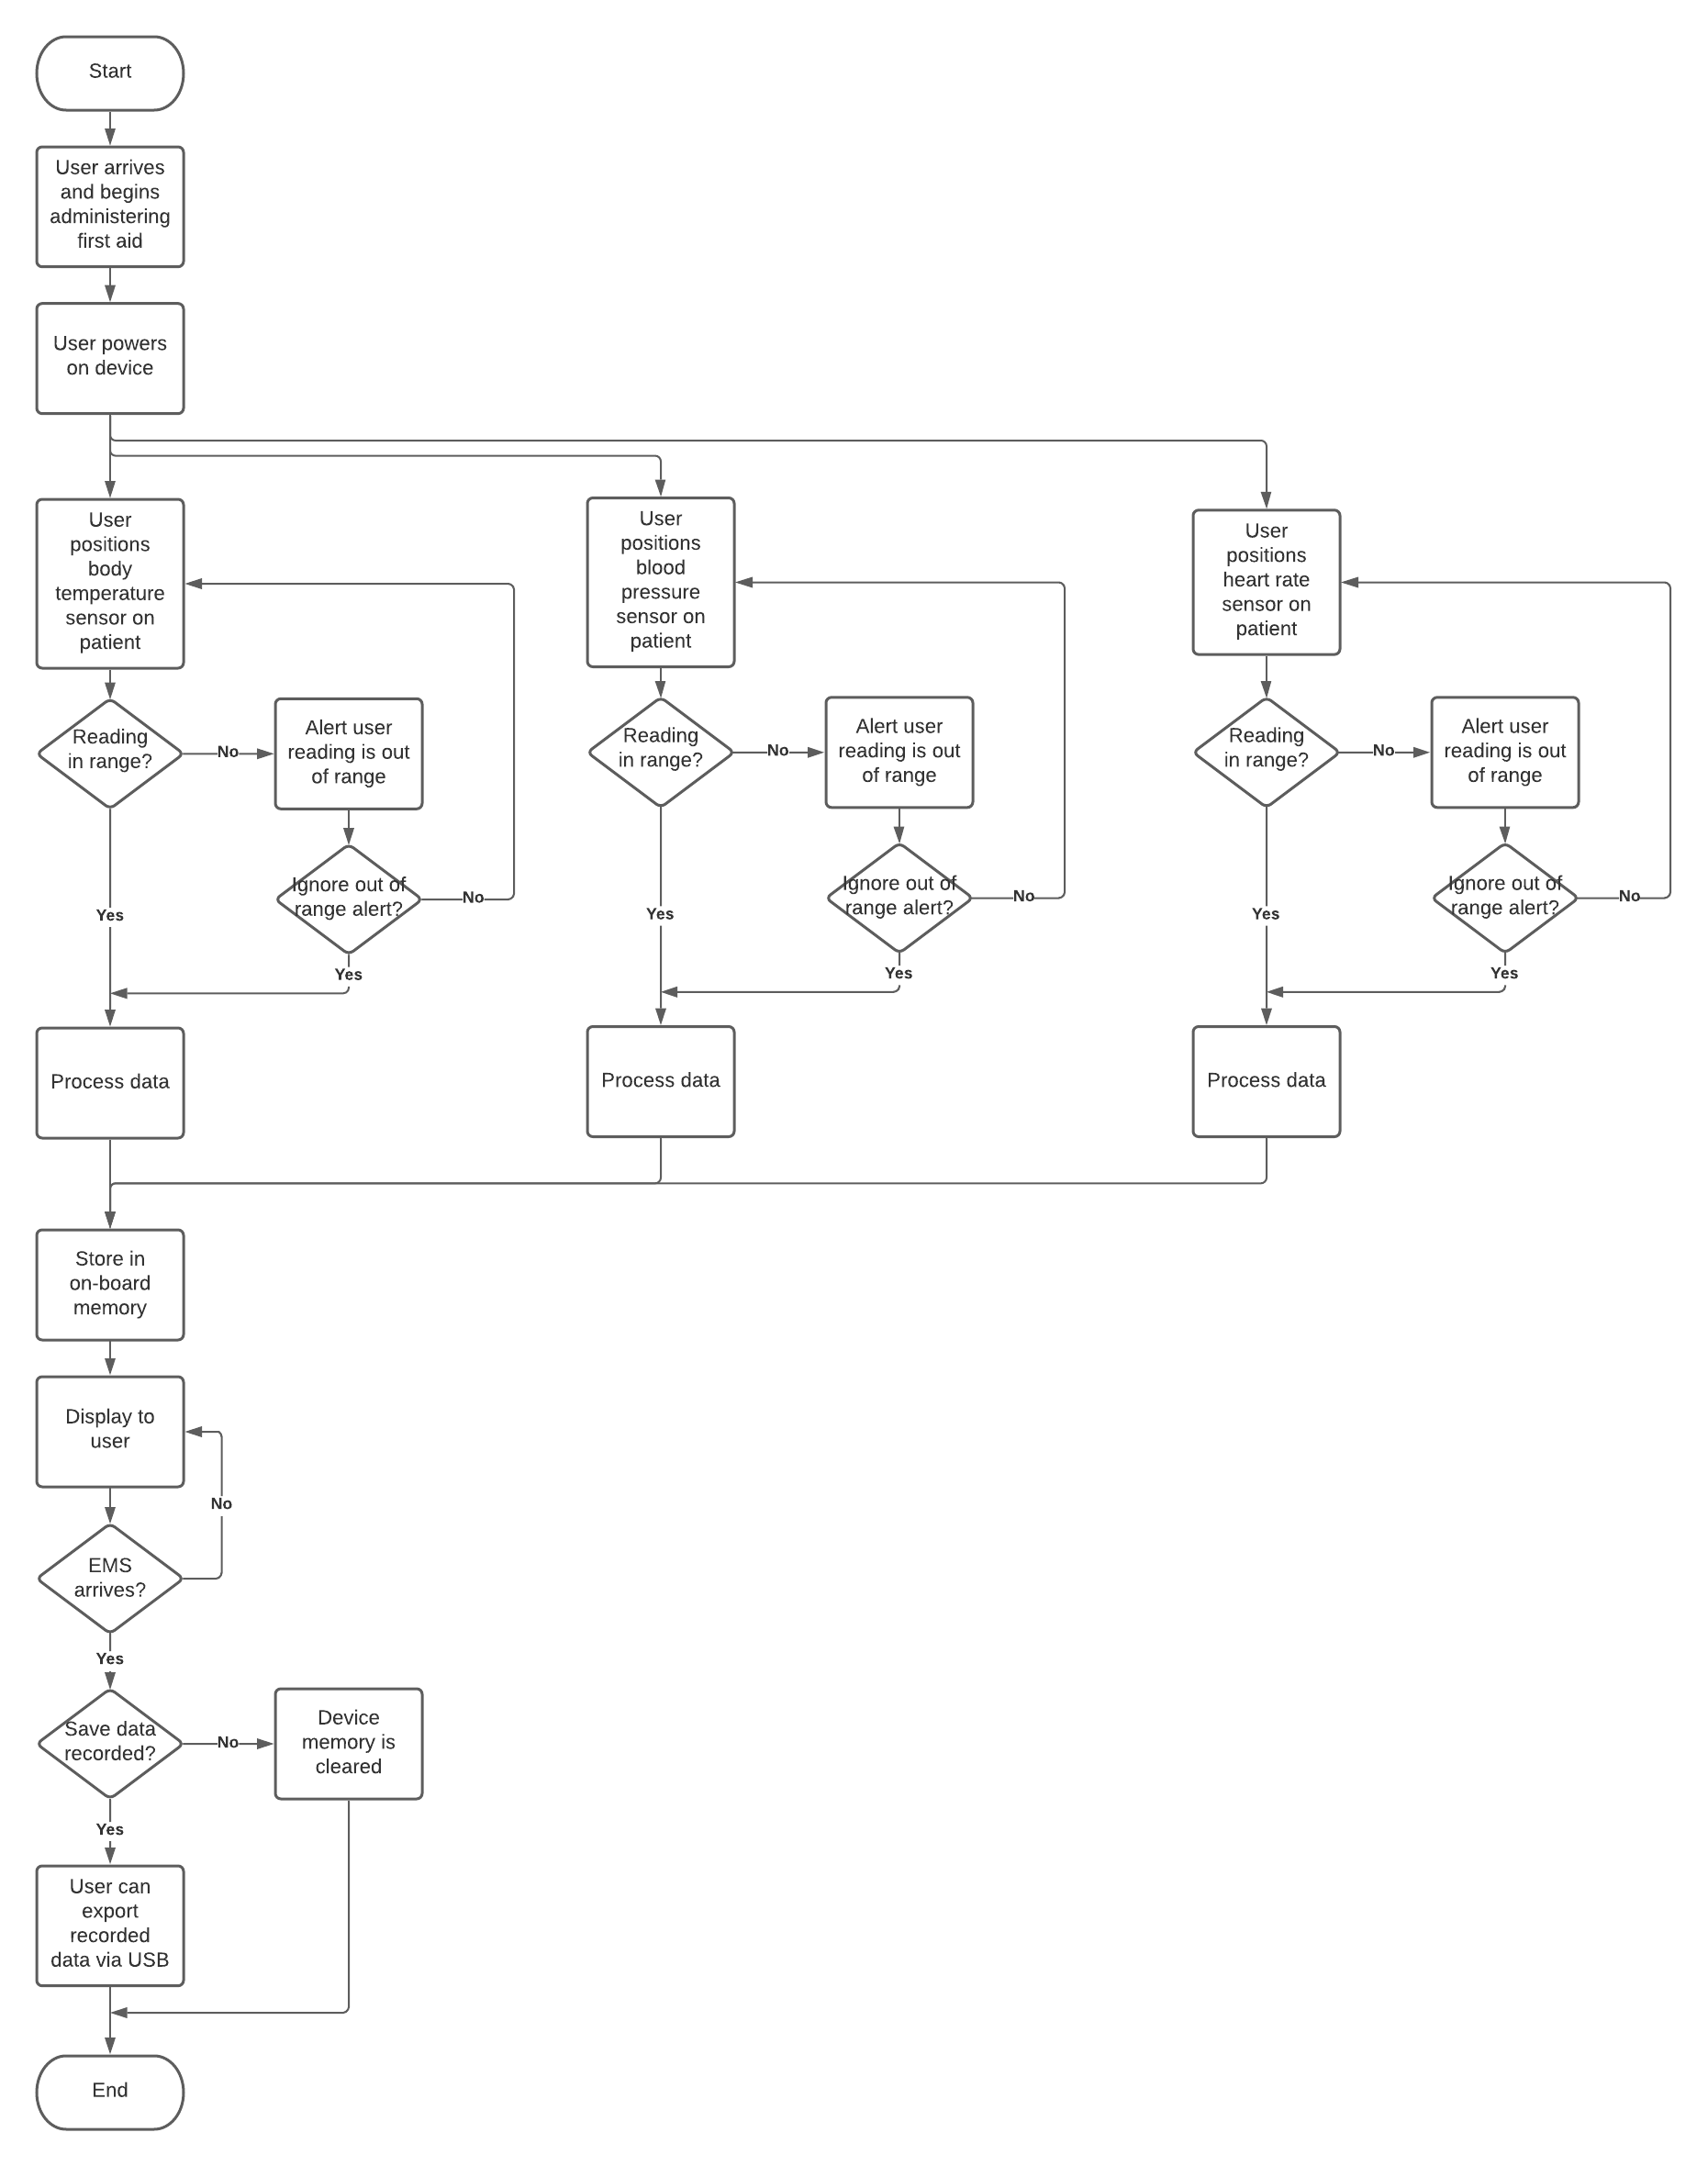
\includegraphics[width=1 \linewidth]{LifeLine block diagrams - Page 3.png}
    	\caption{Flowchart showing how the user interacts with the LifeLine device during normal operation. }
    	\label{flowchart}
    \end{figure}

	\subsection{Undesired Event Handling}
	\subsubsection{Impossible Sensor Values}
	In the event that the sensor readings are outside the possible range for a human the device will inform the user which sensor is giving erroneous readings. The device will recommend that the user ensure the sensor positioning is correct and give them the option to ignore the problematic sensor. 
	
	\subsubsection{Motion Artifacts}
	In the event that the one or more sensors are not securely mounted on the casualty or the casualty is moving, the sensors may return abnormal readings. If these readings are consistently outside of acceptable ranges, the device will warn the user.  However, if the motion artifacts present themselves as sporadic spikes the device will not be able to detect them. It is up to the user to ensure that the sensors are securely mounted on the casualty and that the casualty's movements do not dislodge them.

	\subsubsection{Physiological Noise}
	The sensor readings are expected to have a certain level of noise due to the characteristics of the sensors themselves as well as the variability in the physiological signals that are being read. The device will perform signal processing on data collected from each sensor to smooth out the incoming data however this process is not perfect. A certain level of variability in the data is expected.
	
	\subsubsection{Use in Abnormal Environments}
	Due to the intended use of the device it is expected to be used outdoors where the weather and temperature can vary drastically. That being said extreme heat or cold may impact the accuracy of the sensor readings and the operation of the micro-controller. They may also impact the battery life of the device.The device is also not designed to be submerged under water for long periods of time although it will have some water resistance. The device should be stored in a dry, climate controlled area to ensure consistent operation. 
	
    \subsubsection{Casualty in Undesired Position}
    Depending on the medical situation a casualty may be in a position where it is difficult or impossible to place all sensors correctly on their body and moving them is not an option. Sensors may be placed in a variety of positions on the body and not all sensors need to be placed in order for the device to function, albeit at a reduced capacity. 
    
    \subsubsection{Sensors Obstructed by Dirt or Residue }
    If abnormal sensor readings are detected, the device will inform the user to check that the sensors are not obstructed by any dirt or debris. 
	
	
	\newpage
	\section{Appendix}
	
	\bibliographystyle{plain}
    \bibliography{references}

\end{document}
